\section{Question 8}

Replicate the clusters as given in Figure \ref{Fig: Clusters to replicate}

\begin{figure}
    \centering
    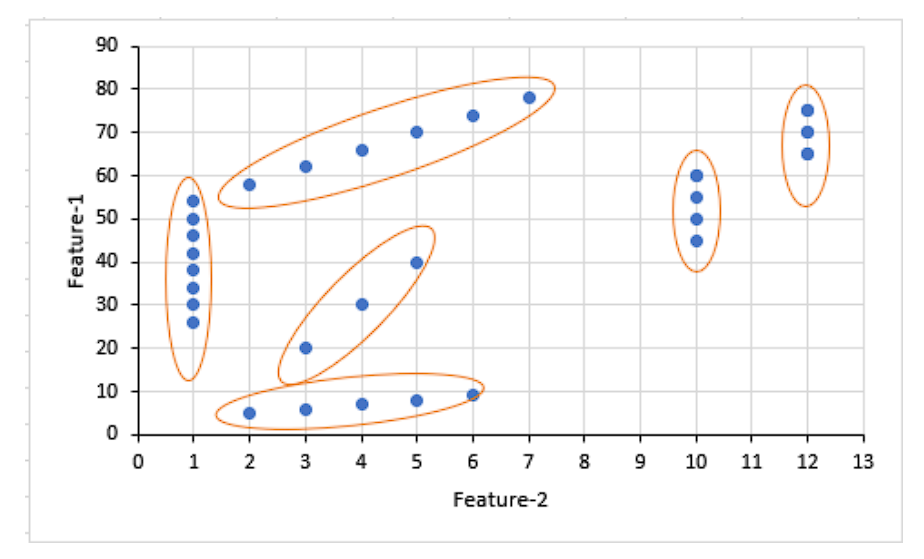
\includegraphics[width=\textwidth]{Appendices/scatter_plot.png}
    \caption[]{Scatter plot with expected clusters (ecliptical shapes)}
    \label{Fig: Clusters to replicate}
\end{figure}

\subsection{Kmean Clustering}
KMeans is a  clustering algorithm athat divide a dataset into $k$ clusters such that the average euclidean distance from a point to the cluster centers.
Hence the KMeans algorithm would not likely to produce the clusters as given in Figure \ref{Fig: Clusters to replicate}.
Instead the Kmeans algorithm with $k=6$ gives the results in Figure \ref{Fig: KMeans6}.

\begin{figure}
    \centering
    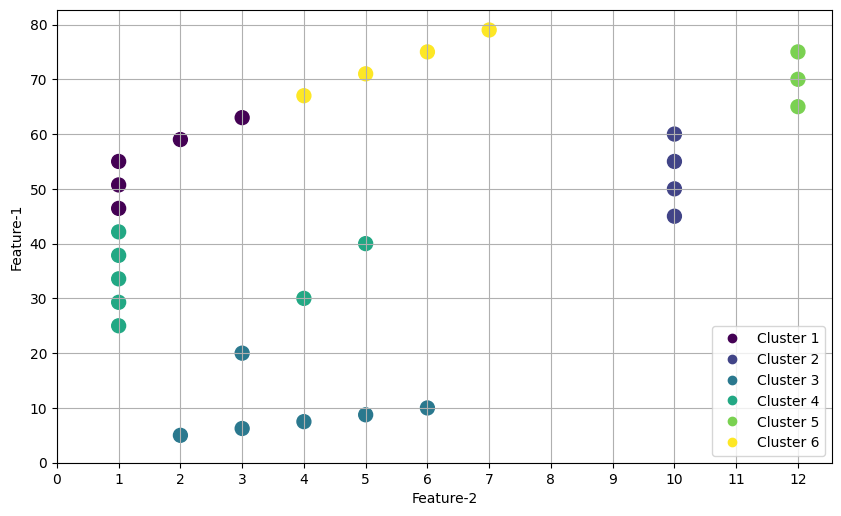
\includegraphics[width=\textwidth]{Appendices/Kmeans6.png}
    \caption[]{Scatter plot with 6 KMeans clusters}
    \label{Fig: KMeans6}
\end{figure}

\subsection{Gaussian Mixture}
Compared to KMeans algorithm, Gaussian Mixture \cite{reynolds2009gaussian} is a model that assumes the distribution of how the data is generated.
Data from Gaussian Mixture model are generally distributed within a spherical or eliptical shape.
Given the clue that the data are fitted within eliptical clusters, we can use Gaussian Mixtrure to identify clusters as given in Figure \ref{Fig: Clusters to replicate}.
The result indeed shows the 6 clusters which matched the desired data (see Figure \ref{Fig: GaussMix6}).

\begin{figure}
    \centering
    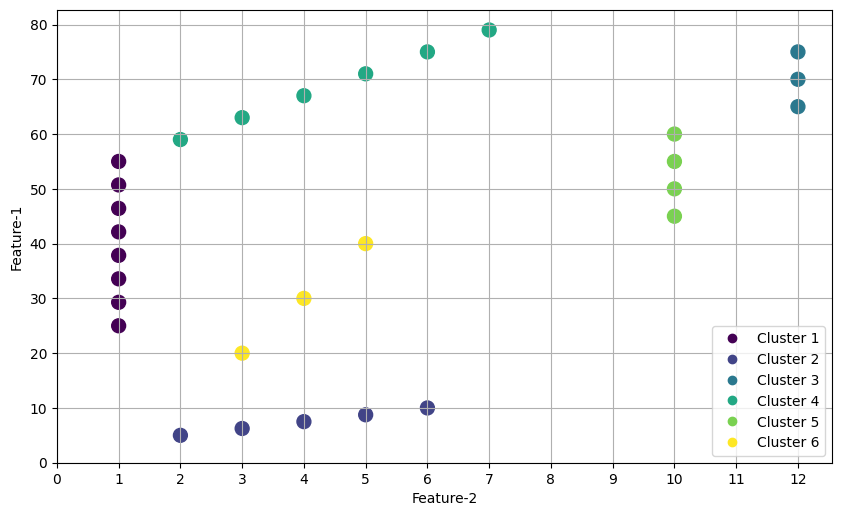
\includegraphics[width=\textwidth]{Appendices/GaussMix6.png}
    \caption{Clustering with Gaussian Mixture model, the data of each cluster matches with Figure \ref{Fig: Clusters to replicate}}
    \label{Fig: GaussMix6}
\end{figure}
